\section{Estado del arte}
\label{sec:StateOfTheArt}
El desarrollo de esta sección se enfoca en dos temas relacionados al
presente trabajo: la comunicación dominio-vista y el manejo de transacciones
dentro de las interfaces de usuario.

\subsection{Estrategias para la comunicación dominio-vista}
La interfaz de usuario necesita obtener información del dominio para presentar
al usuario, así como actualizar esa información a partir de las acciones del usuario.
La necesidad de intercambiar información entre dominio e interfaz de usuario
entra en conflicto con el objetivo de minimizar el conocimiento entre ambas,
como propone el patrón MVC.

Para solucionar esta contradicción la teoría MVC propone que la
comunicación entre dominio y vista se realice a través de eventos. 
Como se explicó en la Sección \ref{sec:Eventos}, los eventos
permiten formas de comunicación con un muy bajo acoplamiento. 
Sin embargo, son pocos los lenguajes que incorporan un manejo automático de
eventos, por eso se requiere utilizar herramientas tecnológicas adicionales.
A continuación detallaremos las estrategias más utilizadas para atacar este problema.

\subsubsection{\emph{Binding} con eventos manuales}
	En algunas tecnologías que no tienen manejo automático de eventos obliga a
	los objetos de dominio a disparar eventos \emph{explícitamente} cada vez cambia
	el valor de una de sus propiedades.
	
	Esta técnica es utilizada en
	frameworks como \emph{JFace-DataBinding}\footnote{JFace-DataBinding es un
	Framework de presentación basado en el lenguaje Java y utilizado para la
	construcción del conocido entorno de trabajo \emph{Eclipse}} y el Arena
	actual, que se basan en el estandar de
	\emph{JavaBean}s \cite{sousa00formal}.
	La figura \ref{javabeans} describe el esquema de eventos utilizado en estas
	tecnologías. El framework lleva un registro de los \emph{listeners}
	interesados en cada propiedad de cada objeto, pero se obliga a cada objeto de dominio a:
	\begin{itemize}
	  \item Tener una referencia a un objeto que actue como soporte para generar
	  los eventos.
	  \item Realizar una notificación cada vez que cambia una de sus propiedades
	\end{itemize} 

	
	 \begin{figure}[h]
		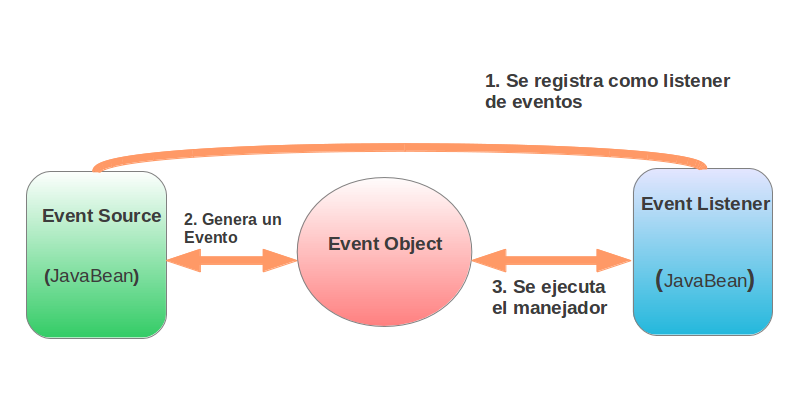
\includegraphics[width=350px, height=200px]{img/javabeans}
		\caption{Esquema de eventos definido por el estándar de \emph{Javabeans}}
		\label{javabeans}
	\end{figure}

	La principal ventaja de esta estrategia es que
	permite una comunicación fluida y desacoplada entre la vista y el modelo.
	El problema es que, al disparar los eventos \\
	manualmente se ensucian las
	clases del dominio. Además, obliga a escribir mucho código repetitivo, que hace que
	sea muy fácil cometer errores.

\subsubsection{Formularios}

	En esta estrategia, durante la edición no se hace un \emph{binding} de los
	datos contra el modelo de dominio. En cambio, se almacenan en un lugar
	intermedio, dentro de la interfaz de usuario, y no hay ninguna comunicación
	con el dominio hasta que el usuario no confirme la acción. En ese momento se
	tranfieren todos los datos juntos, en un único paquete.
	
	Esta estrategia es la forma más tradicional de construcción de aplicaciones
	web. El propio navegador de Internet es el que se ocupa de almacenar los
	datos durante la edición de un \emph{formulario}, que luego se envía
	(\emph{submit}) al servidor. 
	Al recibir este pedido, un componente dentro del servidor se ocupa de desarmar
	el paquete de datos que llega, y transfiere esa información al dominio en forma
	manual.
	
	Una vez procesado el pedido, el servidor contesta con una nueva página que
	el \\ navegador debe presentar al usario, reemplazando por completo la vista
	anterior.\\
	Durante el armado de la página se va pidiendo al dominio cada dato que se desea
	mostrar. Dado que se reemplaza por completo la pantalla del usuario, \textbf{no
	hay necesidad de lanzar eventos} que permitan actualizar lo que el usuario
	estaba viendo.
	
	En aplicaciones de escritorio sin \emph{binding} se puede tener una estrategia
	similar. En lugar de tener un formulario que se envía como un paquete, los
	datos editados se guardan en los propios \emph{controles} de la interfaz de
	usuario. Cuando el usuario confirma la accción, manualmente se toman los datos
	de los controles y se transfieren al dominio.

	\medskip
	
	El problema de esta estrategia es que toda la comunicación debe ser realizada
	en forma manual. Esto es tedioso de mantener y una posible fuente de errores.
	Además, como almacenamos los datos fuera de los objetos de dominio, no podemos
	aprovechar su lógica. Por ejemplo si el objeto de dominio tiene validaciones
	sobre sus atributos, no las podemos aprovechar durante la edición. En
	aplicaciones web tradicionales, muchas veces no se validan los datos hasta que
	no se intenta confirmar la operación, lo que es bastante molesto para el
	usuario. En otros casos, para poder hacer validaciones a medida que el usuario
	edita, la interfaz de usuario tiene su propia implementación de las validaciones. 
	Es decir, la lógica de validación está duplicada.
	 		
\subsection{Manejo de transacciones en la UI}
	Como se explicó en la sección \ref{sec:ACID}, muchas veces las interfaces de
	usuario deben garantizar las propiedades ACID.
	Normalmente las tecnologías que se usan para construir interfaces de usuario no
	tienen soporte nativo para manejar transacciones, entonces el programador se ve
	obligado a implementarlas en forma manual.
	
	Las estrategias más comunes apuntan principalmente a garantizar la atomicidad
	de los cambios. Para ello se evita que la UI interactúe
	directamente con los objetos de dominio. Si la acción que se está realizando
	desde la UI tuviera que modificar un atributo objeto de dominio, el nuevo valor
	del atributo se almacena en algún ``lugar intermedio'' hasta que se confirme toda
	la operación. Esta forma de trabajo simplifica el rollback: simplemente se
	descarta la información intermedia. Los lugares de almacenamiento intermedio
	pueden ser:
	\begin{itemize}
	  \item Un objeto desarrollado específicamente a tal efecto, que sólo tiene los
	  atributos necesarios y ningún comportamiento. \comment{Acá se podría citar
	  http://martinfowler.com/eaaCatalog/dataTransferObject.html, pero del libro,
	  no de la web.}
	  \item Los propios componentes de la interfaz de usuario (por
	  ejemplo una instancia de la clase \texttt{TextBox}).
	  \item En aplicaciones Web, el \emph{request} cubre ese rol.
	  \item Una copia (\emph{clone}) del objeto original.
	\end{itemize}
	
	En cualquiera de estas estrategias, en el momento de confirmar la operación se
	deberá ``trasvasar'' la información del almacenamiento intermedio a los objetos
	de dominio involucrados.
	Con frecuencia esta operación es manual\footnote{En algunos casos puede automatizarse utilizando
	técnicas de \emph{reflection}} e implica una duplicación de conocimiento entre
	el objeto de dominio y el almacenamiento intermedio. Por ejemplo, en caso de
	agregar un atributo al objeto de dominio se deberá garantizar que se mantiene
	sincronizado con los almacenamientos intermedios.
	
	Utilizar una copia del objeto original tiene algunas ventajas sobre las demás
	alternativas. En primer lugar se elimina la duplicación de
	conocimiento, al menos en parte. Por otro lado, esta estrategia permite que la
	UI aproveche el comportamiento del propio objeto durante la edición (por
	ejemplo: validaciones). Además, en esta estrategia hay una variante que se
	utiliza para evitar la trasvasamiento de datos, que es reemplazar el objeto de
	dominio por la copia al final de la operación. Sin embargo, en sistemas
	complejos esta estrategia suele no ser suficiente, porque requiere que podamos
	conocer todas las referencias al objeto que queremos reemplazar. Por otro lado,
	el reemplazo puede muy complejo si la operación modifica múltiples objetos de
	dominio.

	Como se ve, todas estas estrategias logran atomicidad a costa de duplicar
	información y agregar tareas manuales que pueden ser fuente de errores de
	programación. En general no hay una forma sistemática de
	garantizar consistencia o aislamiento.
	
% 	En esta sección analizaremos las estrategias mas utilizadas, y qué propiedades
% 	ACID se cumplen en cada caso.
% 
% 	\subsubsection{Interfaces de Usuario sin estado}
% 		Esta estrategia es muy utilizada en aplicaciones web o en aplicaciones
% 		orientadas a servicios. En este tipo de aplicaciones, 
% 		Se evita almacenar estados en las UIs y se lo delega
% 		todo a la base de datos (BD), o bien debe enviarse en cada interacción con el cliente.
% 		
% 		De esta manera, la	ausencia de datos fuera de la BD, garantiza que no se
% 		rompen estas propiedades.
% 		
% 		Una de las desventajas que tiene este sistema es que si se esta en el
% 		paradigma de la programación orientada a objetos, en cada pedido de datos
% 		se tiene que reconstruir todo el grafo de objetos, y si el grafo es muy grande,
% 		esta operación se vuelve repetitiva y lenta.
% 		
% %		\comment{Otos sistemas que utilizan dicha estrategia son las
% 		% \emph{Arquitecturas orientada a Servicios} y la \emph{Unidad de Trabajo}}
% 		
% 	\subsubsection{\emph{Data Transfer Objects}}
% 		\comment{En este esquema se almacenar la información durante la edición, en
% 		algún lugar fuera del objeto. Como consecuencia se postergan las validaciones de negocio hasta la
% 		finalización de la edición , o se duplica la validación de negocio en la uis.}
% 	
% 	
% 	\subsubsection{Clonar al editar}
% 		Clonar al editar es una estrategia que se basa en la idea de no modificar el
% 		objeto, hasta que se confirme la edición. Cuyo funcionamiento se basa en 
% 		clonar el objeto, y modificar el objeto clonado. Cuando se confirma la
% 		edición, se impacta los cambios del clon en el objeto original.
% 		
% 		Con dicha estrategia la Atomicidad se cumple, ya que solo se pasan los datos
% 		al original, solo cuando se confirma la operación.
% 		En caso de que se quiera cancelar la operación, solo se tiene que tirar la
% 		copia.
% 		
% 		Con el Aislamiento hay problemas si varios usuarios intentan modificar un
% 		objeto, cada uno tendría una copia, pero si mas de uno confirman sus cambios,
% 		los datos quedarían inconsistentes.
% 		
% 		La desventaja que tiene esta estrategia es que se pierde la identidad del
% 		objeto, copiar todos los datos de un objeto a otro, hay que hacerlo a mano,
% y 		esta operación hay que hacerla dos veces, tanto para hacer la copia, y para
% 		confirmar los cambios.
